% PREAMBLE
\documentclass[10pt]{article}

% Packages
\usepackage[usenames]{color}
\usepackage[utf8]{inputenc}
\usepackage{graphicx}
\usepackage{subfig}
\usepackage{url}

% Meta
\author{Joel Mai}
\title{Exposé\\ Framework zum Synchronisieren und Teilen von Inhalten über Peer to Peer}
\date{11. Mai 2021}

% CONTENT
\begin{document}

    \maketitle 

    \newpage

    \section{Einleitung}\label{sec:Einleitung}
    Datenschutz, Privatsspähre, Verschlüsselung. Aktuelle Probleme, die die Menschen zur Zeit beschäftigen. Der alltägliche Datenverkehr wird über die großen Unternehmen ermöglicht und kontrolliert\cite{waandfb2021}. \\ 
    Wer kommunizieren will, muss das meist durch die Abwesenheit von Alternativen über die bereitgestellten Kanäle tun. Die Alternativen die es gibt, sind meist nur rudimentär implementiert oder sperrlich etabliert.
    Sensible Daten, wie zum Beispiel persönliche Erinnerungen, werden unbedacht mit Dritten geteilt. Dabei gibt es schon längst die technlogische Möglichkeit, die Kommunikation über eine verschlüsselte, von fremden Servern unabhängig zu etablieren.\\ Peer To Peer.\\ Meiner Meinung nach, eine viel zu selten genutzte Alternative im Vergleich zu traditioneller Server-Client Verbindungen.

    \section{Problemraum}\label{sec:Problemraum}
    % Was soll warum behandelt werden?
    Das Thema des Praxisprojekts soll das des Entwicklungsprojekts\cite{cobanmai2021} aufgreifen und erweitern. Dabei werde ich mich jedoch nicht sehr an den erarbeiten Inhalten orientieren. Ziel ist es zwar die Idee weiterzuentwickeln, dabei jedoch nicht wieder die selben Fehler und Irrwege zu gehen. So soll das Framework den Austausch von Rezepten über peer to peer ermöglichen und die synchronisierung der Rezepte auf verschiedenen Endgeräten des selben als auch verschiedener Nutzer ermöglichen. Die Vorraussetzung dafür ist es, ein bequemes, nutzerfreundliches Interface und ein System, welches die persistente Datenspeicherung, als auch den sicheren und von großen Unternehmen unabhängigen p2p Austausch ermöglicht. \\
    Gerade diese Punkte wurden für der Prototypen des Entwicklungsprojekts aus Zeitgründen nicht so intensiv behandelt wie erhofft. \\
    Daher ist dieses Mal der erste Schritt, alle notwendigen Kommunikationswege zu erfassen, so wie die Systemschwachstellen zu identifizieren, diese mit bereits bestehenden technologischen Möglichkeiten zu implementieren und auf diesem Framework, das Interface aufzubauen. \\
    Für das Interface ist es besonders ratsam, die bereits erarbeiteten Artefakte zu prüfen und gegebenenfalls zu überarbeiten oder zu ergänzen. Darunter zählen das Domänenmodell, die Nutzermodelle, sowie die erarbeiteten UseCases und Szenarien, die sich sicherlich, mit Abwandelung des zu Grunde liegenden Systems ändern werden. \\

        \subsection{Domänenmodell}\label{sec:Domaenenmodell}
        Das Domänenmodell beinhaltet die ersten rudimentären Änderungen und Abweichungen zu dem Artefakt aus dem Entwicklungsprojekt. Wichtige, für den Problemraum unabdingbare Abläufe werden dort zusätzlich zu den bereits erarbeiteten Domänen erfasst. In Folge dessen, soll die Erarbeitung des Interfaces und dessen Gestaltungslösungen konsquenter umgesetzt werden. Hierbei haltet es sich jedoch nicht um des endgültige Modell, lediglich um eine Momentaufnahme dessen. \\
        Mit * markierte Domänen ergaben sich aus dem vorherigen Artefakt.\cite{cobanmai2021}
        \begin{figure}[h] %!=overrides latex; h=here; t=top; b=bottom; p=special page for floating objects
            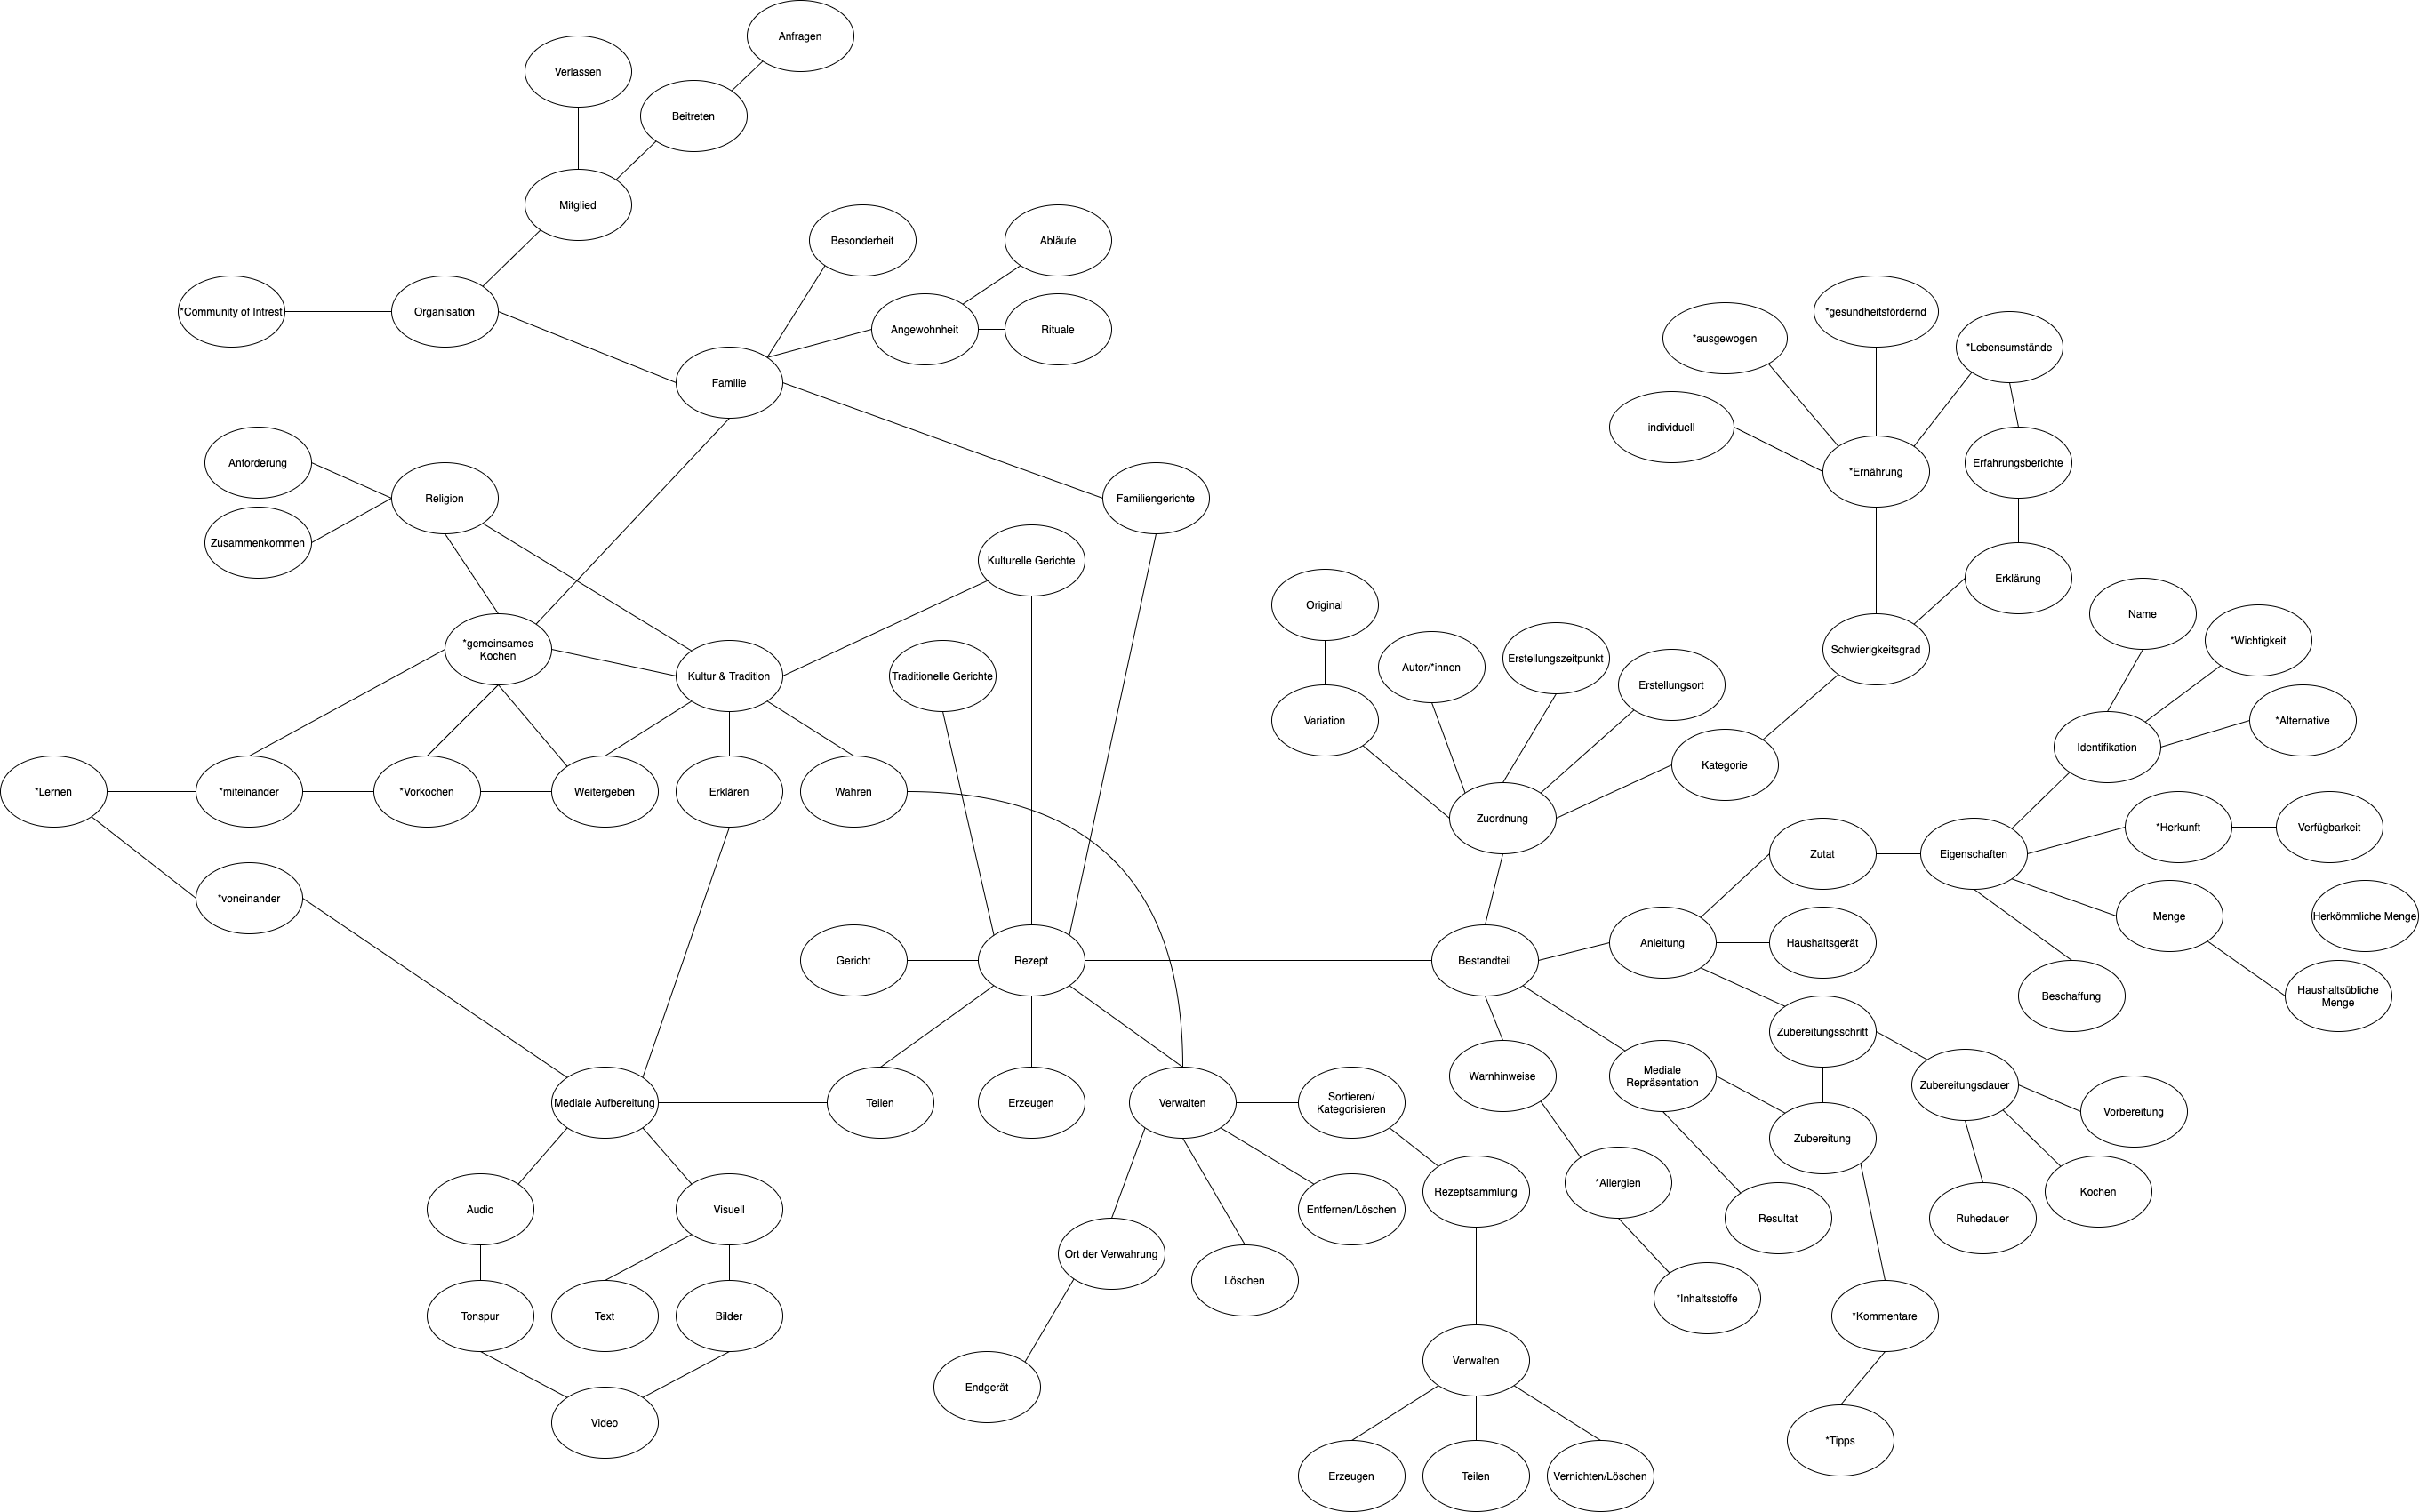
\includegraphics[width=1\textwidth]{../../Domänenmodell/PPSS21_Mai_Domänenmodell.png}
            \caption[Das Domänenmodell]{Domänenmodell, v1}
            \label{fig:domaenenmodell}
        \end{figure}

        \subsection{Problembeschreibung}\label{sec:Problembeschreibung}
        % Existenz und Beschreibung des Problemraums werden durch Quellen belegt
        Das Problem, welches im Praxisprojekt behandelt werden soll, lässt sich in zwei Domänen aufteilen.
            \subsubsection{Kultur- und Traditions-Sharing}\label{sec:cultureandtradition}
            Wollen Menschen untereinander Rezepte austauschen, so gibt es bis her die Möglichkeit eine handgefertigte oder digitale Kopie mit der anderen Person zu teilen. Alternativ könnten sich beide bei gängigen Online Portalen anmelden und dort die Rezepte miteinander, jedoch auch meist mit der Welt teilen. Hier ist zwar das zu Grunde liege Ziel erreicht worden, der Austausch des Rezepts, jedoch können die Nutzer sich hier nur zwischen der Möglichkeit des öffentlichen Teilen aller Informationen oder weniger entscheiden.\cite{gehringirights2021,gelbeseitenrezepte2021} \\
            Gerade in Familien ist es oftmals üblich, dass über die Jahre eine Rezeptsammlung oder gar ein Kochbuch entsteht. Dieses mit den Kindern oder Eltern zu teilen ist oft mit viel bürokratischem Aufwand verbunden, entweder muss das Handschriftliche erst digitalisiert werden oder aufwendig handgefertigte Kopien geteilt werden. Dabei geht der Charm des Erhaltens eines Rezepts der Geliebten verloren.\cite{wohncorerezepte2021} \\
            Nicht zu ignorieren ist auch das Problem des entzifferns oder der verlust sonst nur verbal weitergebener Besonderheiten an einem Rezept. Die Rezept weitergabe erfolgt in vielen verschiedenen Kulturen auf verschiede Art und Weisen, dabei sind die Punkte die für den Erfolg der Weitergabe in der Regel die selben. Es gibt bestimmte Erfahrungsberichte, Tipps oder bestimmte Beschaffungen der Zutaten auf die bei der Zubereitung geachtet werden sollte. Auch die Mengenangaben führen inder Internationalen Küche hin und wieder zu zerlaufenden Keksen. So sind Mengenangaben wie eine Tasse nicht in jedem Haushalt die selbe Menge.\cite{umrechnenbeimbacken2021} \\
            Das einheitliche Anlegen und über die persönlichen Kommentare hinzufügbare Individualisierung würde den Frust aus der Küche nehmen und den Spaß am entdecken der eigenen Kultur fördern. \\
            Ein Rezept ist erstmal ein Rezept, jedoch kann es über die Anreicherung von Medien durch aus zum Leben erweckt werden. Das würde nicht nur den Reiz am Stöbern fördern, aber auch die Familie über geteilte Erfahrungen fördern.\cite{glidzifug2021}

            \subsubsection{Sharing über ein P2P Framework}\label{sec:sharingframework}
            Datenschutz ist wichtig. Bisher gibt es nur wenig Möglichkeiten, Rezepte mit Erinnerungen und Erfahrungen von unterhaltsamen Momenten mit den Engsten anzureichern und diese effizient mit besagten zu teilen. Will man öffentliche Plattformen für diese Zwecke nutzen, so muss man Abstriche bei der Privatsspähre machen. Eine suboptimale Lösung.\cite{weberprivat2021}\\
            Das Speichern besagter Rezepte verläuft meist über selbst angelegte lokale Strukturen oder auf den Servern der Giganten.\cite{tissleraws2021} \\
            Der Austausch der Daten, wenn mindestens über https gesichert, bietet Angriffspotential für duzent weiterer Attaken.\cite{lindauerhttps2021}\\
            Woher weiß der Nutzer im Netz ob die Person mit der er gerade kommuniziert, dass die andere Person auch wirklich die ist, für die sie sich ausgibt.\cite{wbveepcd2021} \\
            Die Organisation der Gruppen in denen Inhalte geteilt werden sollen, sollten die Nutzer selbst anlegen und verwalten können. Das würde ihnen die Freiheit geben zu entscheiden ob nur mit der Familie oder mit ganzen Religionsgemeinden Inhalte geteilt werden sollten, da hier die eigene Tradition und Kultur massiv geprägt wird. \\
            Durch die Erfahrungen des vorherigen Semesters kristalisierte sich die Komplexität von Synchronisierungsabläufen dar. Weshalb in diesem Projekt die Implementierung besondere Zusprüche an Ressourcen erhält. Nutzern soll es schließlich möglich sein, nicht nur an ein Endgerät gebunden zu sein, sondern ihre Inhalte auch auf weiteren Geräten, möglichst ohne Zeitverlust, einsehen zu können. Eine solche Anforderung beinhaltet nicht nur das Teilen von Daten, sondern auch die Verifizierung von Nutzern um vor Datenverlust an Dritte zu schützen.

    \begin{figure}[!h] %!=overrides latex; h=here; t=top; b=bottom; p=special page for floating objects
        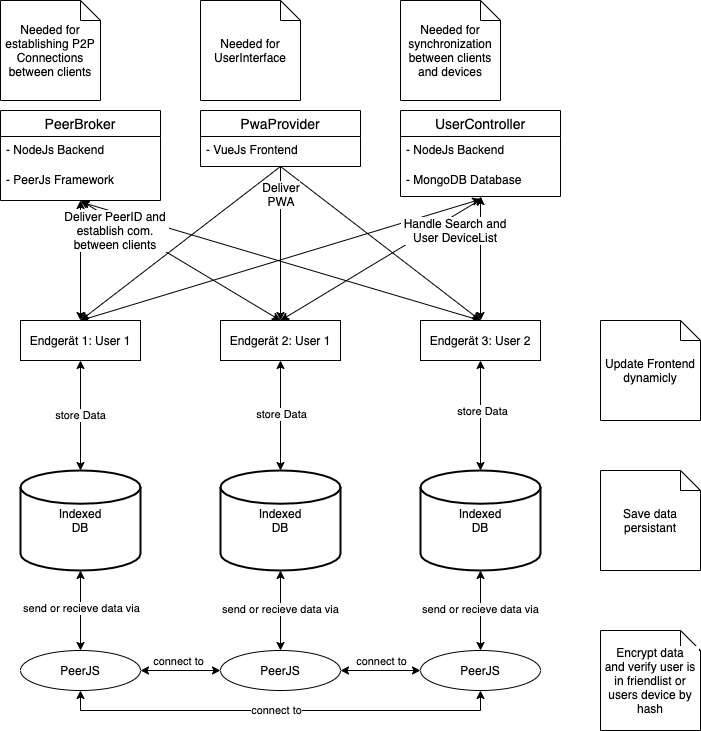
\includegraphics[width=1\textwidth]{../../Systemarchitektur/PPSS21_Mai_Systemarchitektur.jpg}
        \caption[Die Vision]{Systemarchitekturmodell, v1}
        \label{fig:systemarchitekturmodell}
    \end{figure}
    \section{Zielsetzung und Vision}\label{sec:Zielsetzung}
    % Welchen Mehrwert bringt das Projekt und wie erreiche ich diesen?
    % Die Vision ist in der Regel technologieunabhängig; außer sie sind aus dem Problemraum heraus begründet
    % Was soll warum behandelt werden?
    Die genannten Punkte aus \ref{sec:sharingframework} sollen in dem System zu Grunde liegenden Framework angegangen und umgesetzt werden. Daraus resultierend sollen open-source Technologien den umstrittenen Services der Riesenkonzerne vorgezogen werden, und die Implementierung selbst als Open Source Projekt angedacht sein um weitere Generationen motivierter Entwickler anzuregen, neue Wege zu gehen.
    Auf dem Framework selbst sollen die Funktionalitäten eines Rezeptsharing Services implementiert werden und somit eine neue Alternative für das Teilen von Rezepten, in sich selbst verwaltenden Gruppen, entwickelt werden.
    Das Modell \ref{fig:systemarchitekturmodell} zeigt die ersten Ideen zur Umsetzung eines solchen Systems.

    \section{Relevanz}\label{sec:Relevanz}
    % Inwiefern ist die Adressierung dieser bestimmten Problemstellung mittels dieser bestimmen Zielsetzung relevant?
    Datenschutz ist auch heute noch ein akutes Thema, ebenso die Bereitstellung von Frameworks um die Umsetzung interessanter Ideen zu ermöglichen.
        \subsection{Gesellschaftliche Relevanz}\label{sec:Gesellschaftliche}
        % gesellschaftliche Relevanz: trägt zur öko-sozialen Transformation bei
        Familien scheinen sich durch die Digitalisierung immer mehr zu zerstreuen und gemeinsame Erlebnisse scheinen mit dem Alter immer seltener zu werden. Die Wahrung dieser Erlebenisse und das Anregen neue zu erleben ist ohne Frage ein Ziel welches die Gesellschaft zum Besseren bringen würde.\\
        Auch der Schutz des Privatem sollte weiter thematisiert werden. Alternativen zu den gängigen Kommunikationswegen sind immer wieder im Fokus der Presse.

        \subsection{Wirtschaftliche Relevanz}\label{sec:Wirtschaftliche}
        % wirtschaftliche Relevanz: z.B. schließt eine Marktlücke, unterstützt innovative Geschäftsmodelle,
        Open Source Projekte etablieren sich oft nur in Nieschen, dieses hier hätte aber das Potential weitere Projekte dieser Art anzuregen und für mehr Alternativen zu sorgen. \\
        Auch die Bereitstellung eines Sharing Services, welcher sich an Sozialen Netzwerken anlehnt, könnte durch aus das öffentliche Interesse wecken.

        \subsection{Wissenschaftliche Relevanz}\label{sec:Wissenschaftliche}
        % wissenschaftliche Relevanz: bringt einen wissens-orientierten Mehrwert
        Die Weiterentwicklung von P2P hat das Potential weitere Entwicklungen in diesem Bereich der modernen Kommunikation anzuregen. \\
        Es ist wünschenswert die Kommunikation von den Augen neugieriger Dritte abzuwenden und für mehr nutzerorientierter Entwicklung im Web zu sorgen.

    \section{Persönliche Motivation}\label{sec:Motivation}
    Die Implementierung ist mit viel Aufwand verbunden, leider kommt man ohne einen Broker und Provider in der Struktur des Webs nicht aus. Mein Wunsch ist es, ein Framework zu schaffen, welches die Probleme vor denen unser Team letzes Semster stand löst. Ich glaube daran das P2P ein wichtige Alternative ist und es wert ist, dass man sich mit ihr beschäftigt. Auch die Entwicklung eines Nutzerorientierten Interfaces begeistert mich und wird wahrscheinlich mich für den Rest meines Lebens begleiten. \\
    Ich hoffe das Ihnen mein Exposé gefallen hat und Sie mein Interesse teilen.     

    \newpage
    % Bibliothek einbinden
    \bibliographystyle{plain} 
    \bibliography{PPSS21_Mai_Expose.bib}

\end{document}